% Based on a template created by João Alegria (https://github.com/joao-alegria)
%  and Filipe Pires (https://github.com/FilipePires98)

\documentclass[12pt]{article}

\usepackage[english]{babel}
\usepackage[utf8x]{inputenc}

\usepackage{float}
\usepackage{hyperref}
\usepackage{times}
\usepackage{url}

% Images
\usepackage{graphicx}
\graphicspath{{images/}}

% Page dimensions
\topmargin -1.0cm
\oddsidemargin 0.0cm
\textwidth 16cm
\textheight 23cm
\footskip 1.0cm

% TITLE PAGE CONTENT BEGIN

\title{Assignmnet 3}

\author{
    André Pedrosa [85098], João Abílio [84732]\\
    \\
    Recuperação de informação\\
    \normalsize{Departamento de Eletrónica, Telecomunicações e Informática}\\
    \normalsize{Universidade de Aveiro}\\
}

\date{13 de novembro de 2019}

% TITLE PAGE CONTENT END

\begin{document}

\baselineskip18pt

\maketitle

\section*{1. Introdução}
Este relatório apresenta uma explicação do trabalho desenvolvido
para o terceiro assignment da disciplina "Recuperação de Informação",
explicando as decisões tomadas e o funcionamento da solução.

Esta terceira entrega tem como objetivo fazer incrementos à entrega
anterior de maneira a criar uma pipeline que permitia fazer
perquisa sobre o index invertido criado na entrega anterior.

No fim serão apresentados as métricas de eficiência e avaliação dos
resultados devolvidos pelo motor de pesquisa desenvolvido.

Devido ao elevado número de classes criadas, o diagrama de classes
vai ser dividido em vários que vão sendo apresentados ao longo do
relatório. Estes diagramas foram gerados através do IDEA IntelliJ,
consequentemente em anexo é disponibilizada a legenda da convenção
usada.

\section*{2. Data Flow}
\begin{figure}[h]
  \center
  \includegraphics[width=\linewidth]{newsequenceDiagram.png}
  \caption{Diagrama de sequência da solução}
  \label{fig:dataflow}
\end{figure}

O data flow da nossa solução, de modo geral não sofreu grandes
alterações, apenas migramos o código de execução da pipeline de
indexação para uma classe separada, em vez de ser definida na
classe Main.

Na figura \ref{fig:dataflow} está representado sequência de execução
da nossa solução, onde as setas azuis significam que a classe origem
executa um método da classe destino e as setas vermelhas significam
que a classe origem cria a classe destino. Deixando de parte as classes
que têm uma seta vermelha a apontar para si, todas as classes são
instanciadas na classe Main. Na figura existem várias classes em que é
apresentado a classe base e a sua implementação, isto pois algumas
classes base apresentam métodos {\it final} que chamam depois métodos
abstratos que devem estar definidos em classes de descendentes (padrão
Template Method).

\section*{3. Packages}
\begin{figure}[H]
  \center
  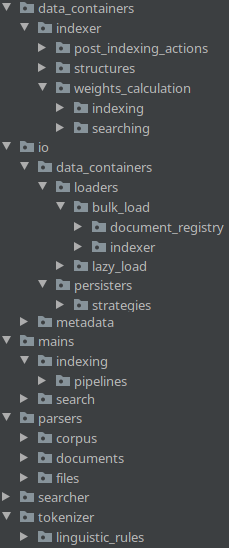
\includegraphics[width=6cm]{packages_all.png}
  \caption{Árvore de packages da solução}
\end{figure}

Nesta secção vão ser apresentadas as alterações feitas a cada package
relativamente à entrega anterior.

\section*{3.1. tokenizer}
\begin{figure}[H]
  \center
  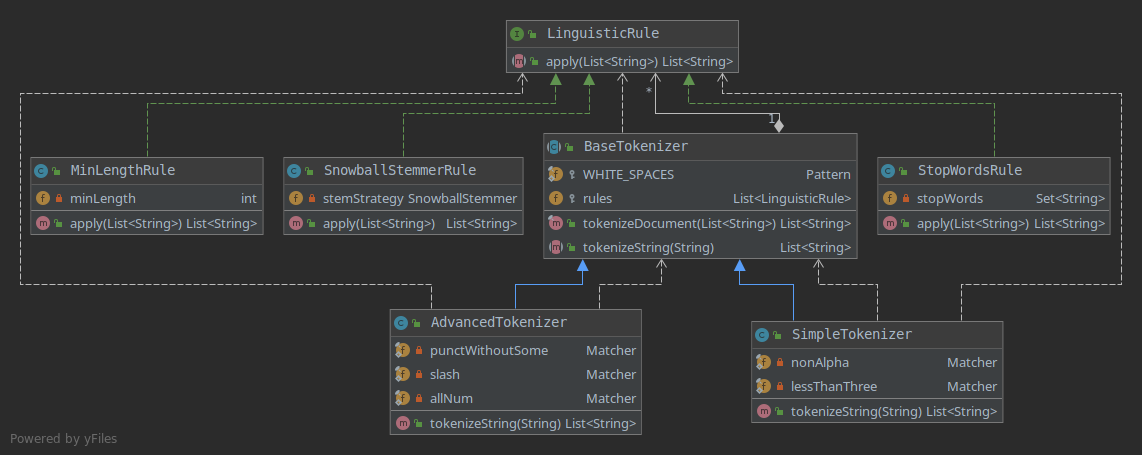
\includegraphics[width=\linewidth]{packages_tokenizer.png}
  \caption{Diagrama de classes do package \it tokenizer}
\end{figure}

Este package também não sofreu alterações relativamente à
entrega anterior.

\section*{3.2. parsers}
\begin{figure}[H]
  \center
  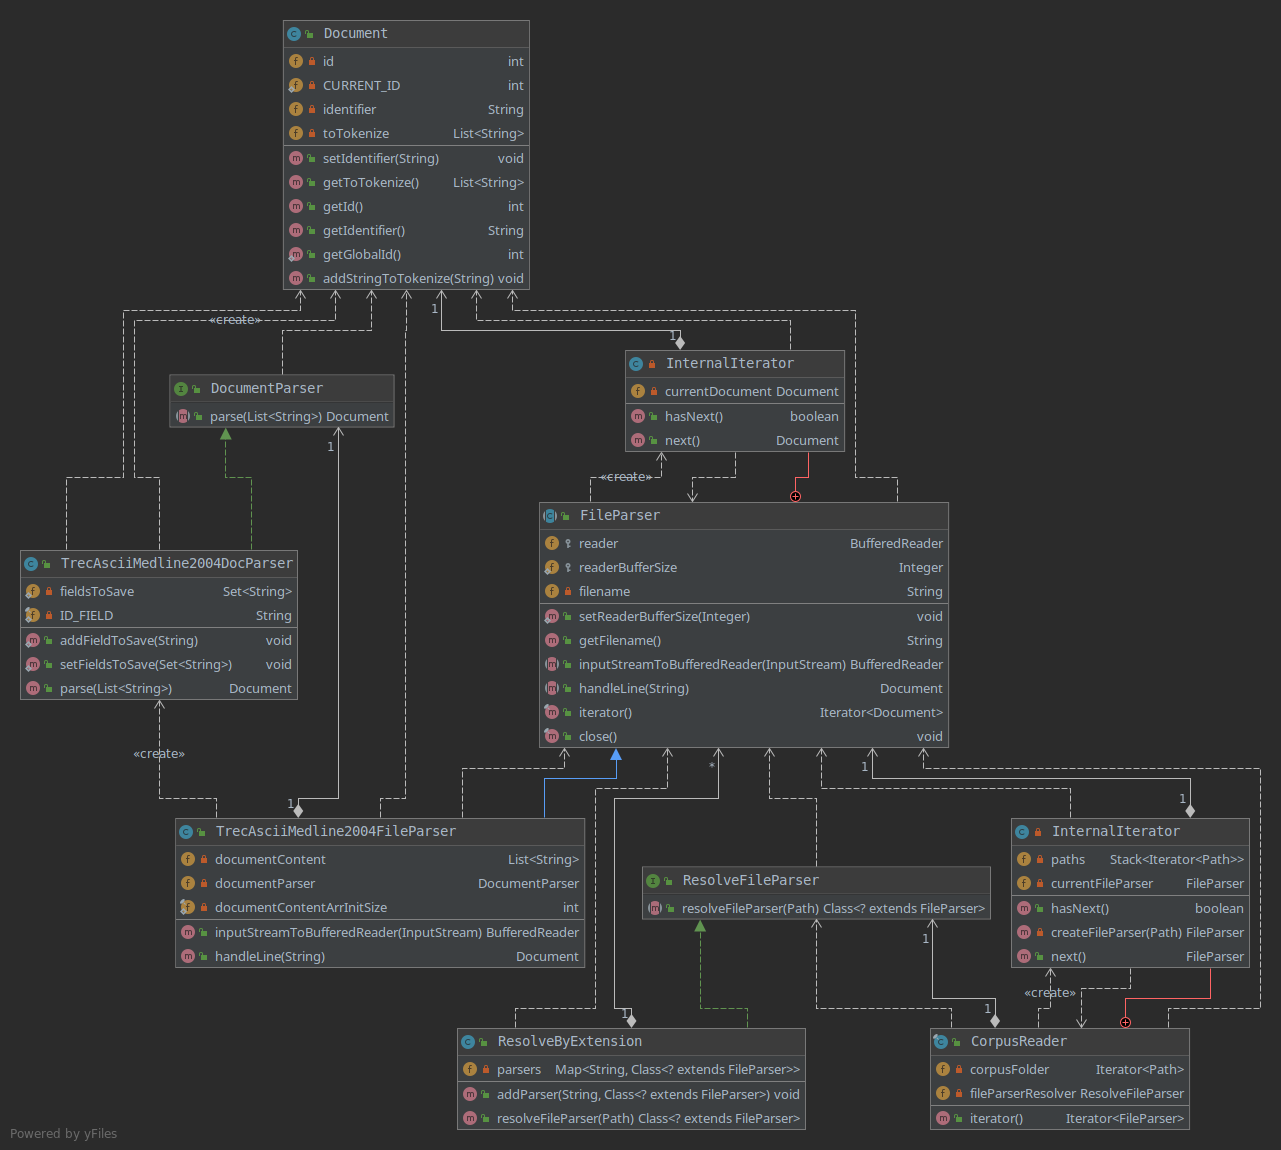
\includegraphics[width=\linewidth]{packages_parsers}
  \caption{Diagrama de classes do package \it parsers}
\end{figure}

Este package não sofreu grandes alterações relativamente à entrega
anterior, apenas foi alterado o tipo de dados do identificador
original de cada documento de {\it String} para {\it int}.

\section*{3.3. data\_containers}
Na entrega anterior tanto o inverted index como o document registry
estavam presentes na mesma classe, Indexer.
Isto trazia alguns problemas para a pipeline de responder a queries
pois quando o inverted index era carregado o respetivo document
registry devia também de ser carregado.
No entanto um termo pode ter um documento de id 1, que foi o primeiro
a ser indexado, e outro com id 4.000.000, um dos últimos a serem
indexados.
Isto implicava consultar diferentes segmentos do document registry já
em disco na altura de indexação, isto supondo que não todos em
memória.

Com isto em consideração separamos o document registry e o indexer em
duas classes, o Indexer que contem o inverted index (Map) e o
DocumentRegistry que contem a tradução entre o nosso identificador
interno com o identificador original (Map).
É de realçar que estas classes apenas serão usadas em tempo de
indexação.

\section*{3.3.1. data\_containers.indexer}
\begin{figure}[h]
  \center
  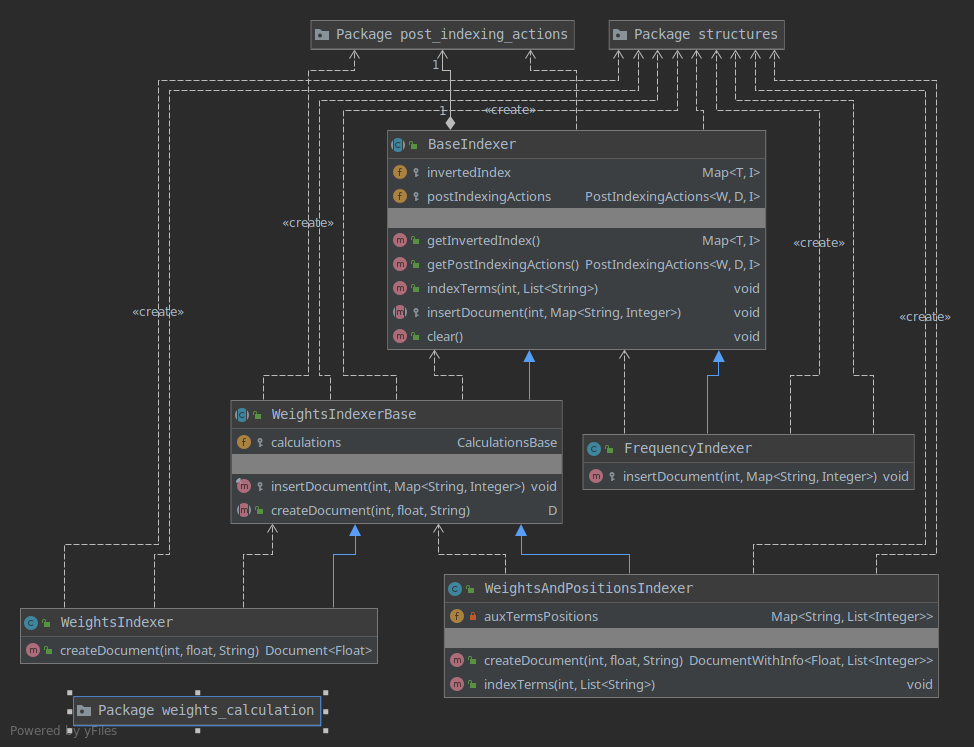
\includegraphics[width=\linewidth]{packages_data_containers_indexer.png}
  \caption{Diagrama de classes do package \it
    data\_containers.indexer}
\end{figure}

Este package sofreu algumas alterações, no entanto as alterações
foram feitas mais ao nível dos sub packages o que levou a adaptações
depois das classes presentes na root deste package.

\section*{3.3.1.1 data\_containers.indexer.post\_indexing\_actions}
\begin{figure}[h]
  \center
   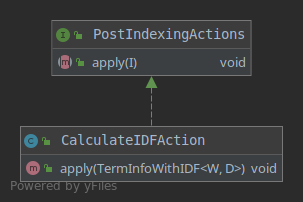
\includegraphics[width=6cm]{packages_data_containers_indexer_post_indexing_actions.png}
  \caption{Diagrama de classes do package \it
    data\_containers.indexer}
\end{figure}

Como na entrega anterior o pesos dos documentos estavam a ser mal
calculados, estando a ser calculados por termos em ver de por
documentos, a {\it post indexing action} criada agora apenas calcula
o idf dos termos, que apenas pode ser calculado no final do processo
de indexação.

\section*{3.3.1.2 data\_containers.indexer.structures}
\begin{figure}[H]
  \center
   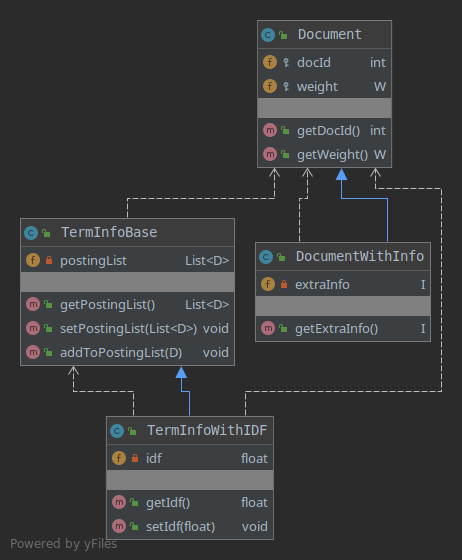
\includegraphics[width=7cm]{packages_data_containers_indexer_structures.png}
  \caption{Diagrama de classes do package \it
    data\_containers.indexer.structure}
\end{figure}

Neste package temos as estruturas que vão ser usadas para armazenar a
informação relativa aos documentos indexados no inverted index.

Este package sofreu algumas alterações devido ao facto de em entregas
anteriores objetos com informação serem usados como chave do inverted
index e esta ser necessária posteriormente na fase de pesquisa. Mais
concretamente falamos do objeto Term em que usávamos o termo para
gerar o hashcode e também para comprar objetos Term para depois ser
inserido em HashMaps ou ordenados respetivamente.

Um exemplo de informação extra que era guardada no objeto Term era o
idf de um termo. No entanto para obter este teríamos de percorrer
todas as chaves do HashMap até encontrar aquela que tinha o termo
igual ao que queríamos obter o idf. Isto é uma operação $O(n)$, ou
seja, estávamos a perder o tempo constante de acesso a um HashMap.

De maneira a corrigir o problema apenas definimos objetos para os
valores associados a um termo indexado, ou seja, os valores de um
HashMap. Estes valores são do tipo {\it TermInfoBase} que contêm
sempre uma posting list de documentos. Cada documento tem sempre um
id e um peso associado. Podem ainda existir subclasses da classe {\it
TermInfoBase} que podem ter outras informações como o idf (objeto
{\it TermInfoWithIdf}) e os documentos podem também ter outras
informações associadas como as posições (objecto {\it
DocumentWithInfo}).

\section*{3.3.1.3 data\_containers.indexer.weights\_calculation}
\begin{figure}[H]
  \center
   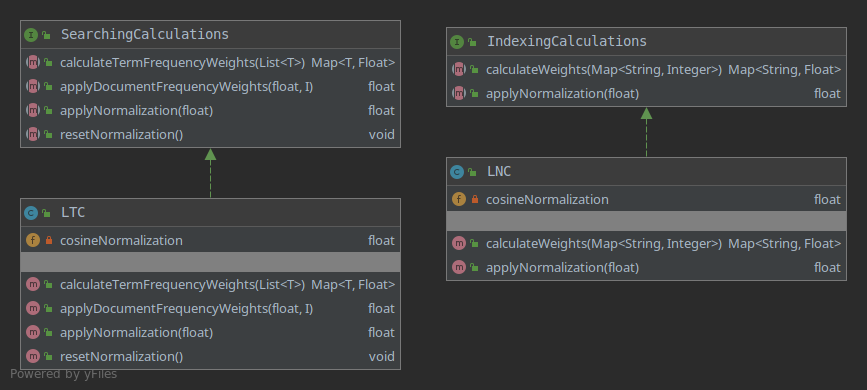
\includegraphics[width=\linewidth]{packages_data_containers_indexer_weights_calculation.png}
  \caption{Diagrama de classes do package \it
    data\_containers.indexer.weights\_calculations}
\end{figure}
asdfsdf

\section*{3.4. io}
\section*{3.4.1 io.metadata}
\section*{3.4.2 io.data\_containers}
\section*{3.5. searcher}
\section*{3.6. mains}


Como foi dito na secção anterior, o código de execução da pipeline
de indexação que estava presente na classe Main, foi migrado para
para uma classe do tipo Pipeline. Ou seja, a classe Main apenas
tem a responsabilidade de instanciar as classes necessárias para
a execução da pipeline.

\subsubsection{pipelines}

Este package tem as classes que definem a sequência de execução
do método de indexação. A classe principal (Pipeline) está encarregue
de iterar sobre o corpus e passar cada FileParser à implementação
de Pipeline escolhida (método processFile) e depois disso executar
o método para persistir o indexer.

A classe SimplePipeline representa a pipeline que foi definida no
assignment anterior, em que não tem considerações relativamente à
memória no processo de indexação. A SPIMIPipeline apresenta uma
implementação em que o método de indexação é feito segundo o
algoritmo SPIMI, em que durante a indexação, sempre que a memória
ocupada chegar a um limite (80\% da memória máxima), o index atual
é escrito para disco, ordenado pelos termos. De maneira a criar um index
final, esta pipeline faz um merge dos vários ficheiros criados na
fase anterior. Este merge é feito lendo blocos (implementado com a
classes que usam métodos de buffering enquanto lêm, como por exempo
BufferedInputStream e BufferedReader) de todos os ficheiros temporários
criados. Para fazer merge destes blocos, é mantida uma lista à qual é
adicionada iterativamente a entry (termo e posting list) em que o termo é
menor (alfabeticamente) de entre as várias entries lidas dos vários
ficheiros temporários a fazer merge. Caso haja o mesmo termo em
diferentes blocos é feito o merge das posting lists segundo os
document ids.

Os ficheiros temporários foram escritos em binário (usando a classe
ObjectOutputStream), já que se revelou ser muito mais rápido do que
aplicar a forma de persistência que o utilizador escolhe no Main, no
caso deste assignment CSV. Para guardar o index final foram criados
vários ficheiros, tendo cada um um número máximo de entries e para
saber quais os termos presentes em cada ficheiros deste foi inserido
como sufixo ao nome dos ficheiros o primeiro termo que guardam.

A classe indexer, para além de guardar o index invertido, guarda também
o document registry que contêm a associação entre um document id, gerado por nós cada vez que um documento é criado, e o identificador presente nos
documentos, no caso deste corpus o campo PMID. Como a geração deste id é incremental e não existem vários documentos com o mesmo document id, na
altura da indexação, quando a memória atingir o limite máximo, podemos
já escrever esta estrutura num ficheiro final. A maneira como esta
estrutura será persistida vai ser explicada mais à frente no package
indexer.persisters.

\subsection{indexer}

Este package foi o que sofreu mais alterações relativamente à entrega
anterior. Foram criados novas classes indexer (árvore de classes
WeightsIndexerBase) que guardam pesos tanto para o termos como
para os documentos presentes nas posting lists. Foi criado também
um novo package, post\_indexing\_actions, que contêm classes que
aplicam sobre cada entry do indexer ações depois do processo de
indexação e antes de serem persistidos de modo final, ou seja, no
caso da pipeline que aplica o algoritmo SPIMI, estas ações apenas
serão aplicadas quando uma entry estiver pronta para ser escrita
para o ficheiro do index final, por outras palavras, depois das
posting lists dos termos iguais presentes nos vários ficheiros
temporários serem combinadas. Cada indexer tem uma classe
post\_indexing\_action especifica associada. Por fim, foi feito
um refactor relativamente à persistência das estruturas internas
do indexer.

\subsubsection{indexer.structures}

Deste subpackage foram removidos as classes especificas de termos ou
documentos, por exemplo um documento com frequência é criado com uma
classe BlockWithInfo que implementa a interface BaseDocument em que o
tipo da extraInfo da classe BlockWithInfo é Integer. Para criar um
documento com weight (float) teria de criar um uma outra classe
semelhante à anterior mas o tipo da extraInfo seria do tipo Float.
Para evitar isso criou-se as quatro combinações das classes Block
(Block e BlockWithInfo) com as classes BaseTerm e BaseDocument.

O package aux\_structs contêm classes a serem usadas no campo
extraInfo das classes descendentes da classe BlockWithInfo. A
duas classes representadas são usadas como extraInfo dos documentos
dos indexers que calculam weights para termos e documentos.

\subsubsection{indexer.io.persisters}

Como as estruturas internas do indexer são mapas, desenvolvemos uma
nova versão dos persisters em que as classes bases (BasePersister)
iteram sobre as as entries (key:value) ordenadas pela key, e as
classes descendentes devem implementar o modo como cada entry é
escrita para disco. Nos implementamos dois modos de persistência,
um usando uma ObjectOutputStream e outro usando uma OutputStream.
A primeira escreve as entries como objectos Map.Entry e o segundo
escreve a representação da key em bytes, um separador, a
representação do value em bytes e um terminador. Este ultimo tipo
de persister implica defenir uma OutputStreamStrategy que define
a estratégia de transformar as keys e values em bytes. No caso da
estrutura inverted index do indexer estas estratégias (árvore de
classes IndexerStrategy) transformam um termo em bytes e cada
documento das posting lists também em bytes (Criam uma String
com um determinado formato e devolvem os bytes dessas Strings).

Como os ficheiros escritos são sequenciais, ou seja, para aceder
a uma parte algures do ficheiro é necessário ler todo o ficheiro
até à posição especifica. Para tentar reduzir a leitura a ficheiros
a disco, cada estrutura interna do indexer vai ser escrito para
vários ficheiros em que cada ficheiro tem um numero máximo de
entries. Os nomes destes vários ficheiros é a concatenação do
prefixo definido pelo utilizador mais um contador e a representação
em string da primeira key guardada nesse ficheiro. O contador é
usado pois no caso da indexação inicial do algoritmo SPIMI, vários
ficheiros podem vir a ter o mesmo termo como primeiro termo.

\subsubsection{indexer.io.loaders}

Como os persisters escrevem entries uma a uma, para criar os loaders
usamos iteradores para ler dos ficheiros. A classe base, BaseLoader,
definea estrutura básica do iterador o qual as classes descendentes
devem completar pois a leitura de entries depende do método de
escrita e da estratégia usada. Criamos duas implementações de
loader, ObjectStreamLoader que lê objetos entry e o ReaderLoader que
lê linha a linha. Este último tem depois uma strategy que transforma
um linha num objeto Map.Entry. Como neste assignment ainda não é
necessário fazer load do index final, não foram implementados
strategies especificas para cada indexer.

\subsubsection{indexer.post\_indexing\_actions}

Neste package encontram-se definidas ações para serem executadas
sobre as vários entries da estrutura inverted index dos indexers,
depois do processo de indexação e antes de a versão final ser
persistida para disco. O objetivo principal é realizar cálculos
que apenas podem ser feitos no fim de ter passado por todos os
documentos do corpus, os quais são o calculo do idf de cada termo
(depende do número total de documentos) e a normalização dos pesos
dos documentos para cada posting list (apenas pode ser calculado
quando a posting list estiver completa). De maneira a conseguir
calcular estes pesos, durante a indexação é calculado a frequência
de cada termo para cada documento, o que depois permite calcular
o idf para cada termo e o peso do termo para cada documento.

\newpage

\section{Resultados}

Resultados usando os dois ficheiro 2004\_TREC\_ASCII\_MEDLINE gz,
não fazendo nenhuma limitação da memória através da JVM,  no
inicio da execução do programa havia por volta de 4GB de memória
disponível, escritas e leituras  para o disco foram feitas sobre
um HDD e o CPU i5-6300HQ CPU @ 2.30GHz.

{
\tiny
\begin{tabular}{| c | c | c | c | c | c | c | c |}
        \hline K
        & \bf  Média precision
        & \bf  Média recall
        & \bf  Média F-measure
        & \bf  Média Average Precision
        & \bf  Média NDCG
        & \bf  Query throughput
        & \bf  Query latency \\

        \hline 10
        &
        &
        &
        &
        &
        &
        & 1 \\

        \hline 20
        &
        &
        &
        &
        &
        &
        & 1 \\

        \hline 50
        &
        &
        &
        &
        &
        &
        & 1 \\
        \hline

\end{tabular}
}

\newpage

\section{Anexos}

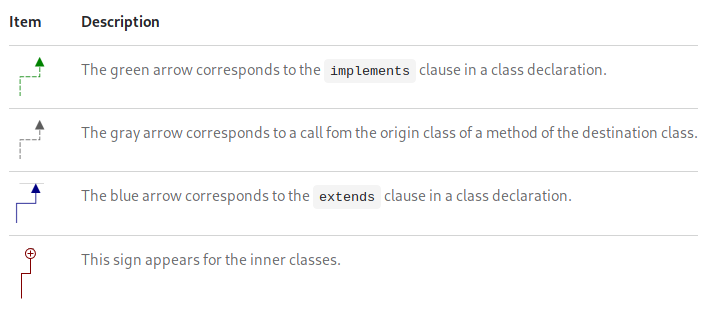
\includegraphics[width=13cm]{arrow_legend.png}

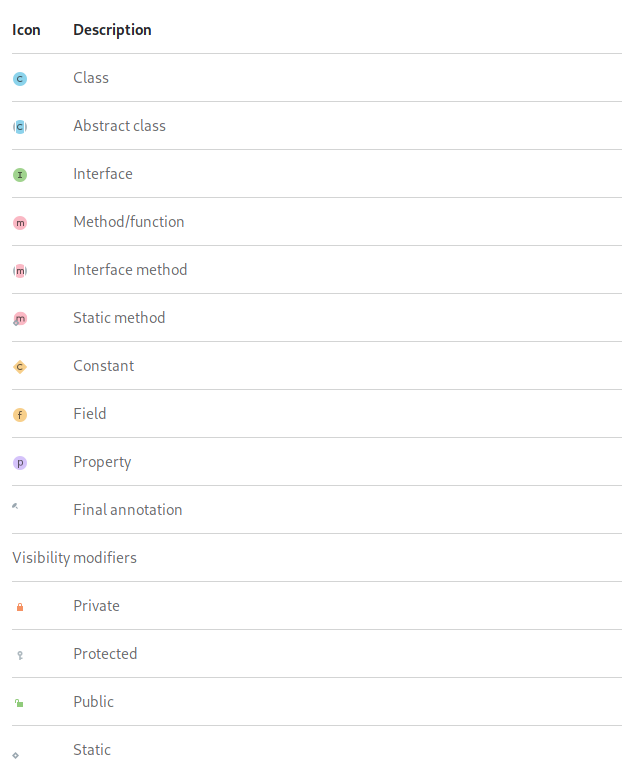
\includegraphics[width=13cm]{icons_legend.png}

\end{document}
